\newpage

\section{Quadro economico di progetto}
Si elenca, di seguito, il prospetto economico per il progetto: esso è suddiviso in sezioni riguardanti ciascuna fase dello stesso. Il piano economico così presentato, si basa sul calcolo delle ore presentato in precedenza. Sarà inserita, per scopo puramente conoscitivo, anche la fase di Analisi dei Requisiti, nonostante non sia rendicontabile e non rientri, quindi, nel calcolo complessivo. Di seguito, si illustrano i valori di riferimento per il calcolo dei costi:

\begin{table}[H]
	\begin{center}
		\begin{tabular}{|c|c|}
			\hline
			\textbf{Ruolo}	& \textbf{Costo per ora} \\
			\hline
			\Res	&	30	\\
			\hline
			\Amm	&	20	\\
			\hline
			\Ana	&	25	\\
			\hline
			\Prog	&	22	\\
			\hline
			\Progr	&	15	\\
			\hline
			\Ver	&	15	\\
			\hline
		\end{tabular}
	\end{center}
	\caption{Costo per ora, suddiviso per ruolo}
\end{table}

\newpage
\subsection{Analisi dei Requisiti}

Il periodo di Analisi dei Requisiti è parte dell'investimento intrapreso dal gruppo \textit{\gruppo} per la realizzazione del progetto \progetto. Come si evince dalla tabella sottostante, il costo è interamente a carico del team. Il prospetto economico per quanto concerne l'Analisi dei Requisiti è il seguente:


\begin{table}[H]
	\begin{center}
		\begin{tabular}{|c|c|c|c|}
			\hline
			\textbf{Ruolo}	& \textbf{Numero di ore} & \textbf{Costo} & \textbf{Costo a preventivo} \\
			\hline
			\Res	&	38  &	1140 &  0	\\
			\hline
			\Amm	&	11  &	220  &  0	\\
			\hline
			\Ana	&	79  &	1975 &  0	\\
			\hline
			\Ver	&	61  &	915 &  0	\\
			\hline
			\textbf{Totale}  &	\textbf{189}	& \textbf{4250}  &  \textbf{0}	\\
			\hline
		\end{tabular}
	\end{center}
	\caption{Prospetto dei costi, Analisi dei Requisiti }
\end{table}

\begin{figure}[H]
	\centering
	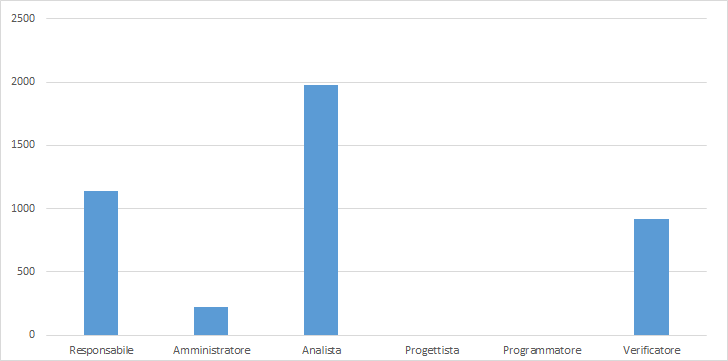
\includegraphics[scale=0.6]{img/8-1.png}
	\caption{Incidenza costi, Analisi dei Requisiti}
\end{figure}

\newpage
\subsection{Analisi dei Requisiti Dettagliata}
Anche il periodo di Analisi dei Requisiti Dettagliata fa parte dell'investimento del gruppo \textit{\gruppo} per la realizzazione del progetto \progetto. Come nel caso precedente, il costo è interamente a carico del team. Il prospetto economico riguardante l'Analisi dei Requisiti Dettagliata è il seguente:


\begin{table}[H]
	\begin{center}
		\begin{tabular}{|c|c|c|c|}
			\hline
			\textbf{Ruolo}	& \textbf{Numero di ore} & \textbf{Costo} & \textbf{Costo a preventivo}\\
			\hline
			\Res	&	4  &	120 &  0	\\
			\hline
			\Amm	&	1  &	20 &  0	\\
			\hline
			\Ana	&	5  &	125 &  0	\\
			\hline
			\Ver	&	5  &	75	&  0	\\
			\hline
			\textbf{Totale}  &	\textbf{15}	&  \textbf{340}	 &  \textbf{0}	\\
			\hline
		\end{tabular}
	\end{center}
	\caption{Prospetto dei costi, Analisi dei Requisiti Dettagliata }
\end{table}

\begin{figure}[H]
	\centering
	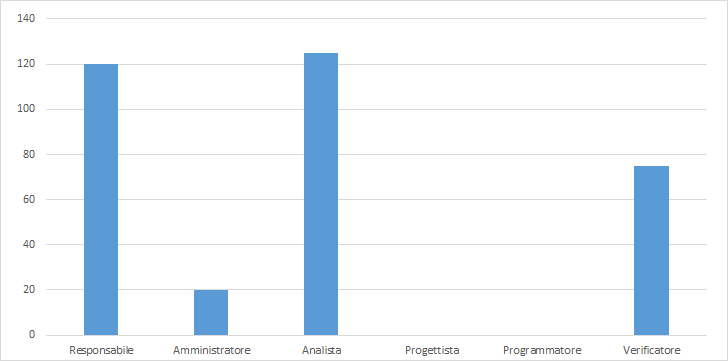
\includegraphics[scale=0.6]{img/8-1a.png}
	\caption{Incidenza costi, Analisi dei Requisiti Dettagliata}
\end{figure}

\newpage
\subsection{Progettazione Architetturale}
Il prospetto economico per quanto concerne la Progettazione Architetturale è il seguente:


\begin{table}[H]
	\begin{center}
		\begin{tabular}{|c|c|c|c|}
			\hline
			\textbf{Ruolo}	& \textbf{Numero di ore} & \textbf{Costo} & \textbf{Costo a preventivo} \\
			\hline
			\Res	&	5  &	150  &	150	\\
			\hline
			\Amm	&	5  &	240  &	240	\\
			\hline
			\Prog	&	138  &	3036  &	3036	\\
			\hline
			\Ver	&	52  &	780  &	780	\\
			\hline
			\textbf{Totale}  &	\textbf{200} &	\textbf{4206} &	\textbf{4206}	\\
			\hline
		\end{tabular}
	\end{center}
	\caption{Prospetto dei costi, Progettazione Architetturale }
\end{table}

\begin{figure}[H]
	\centering
	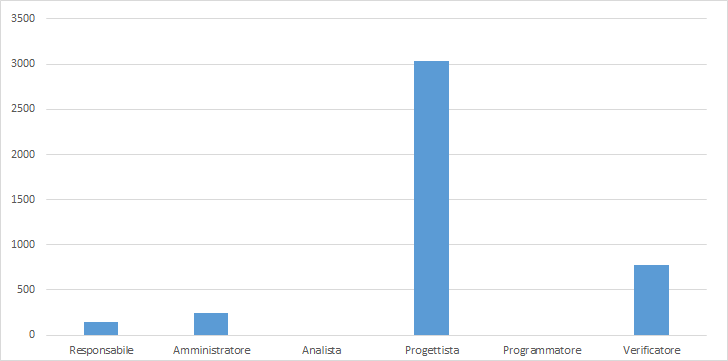
\includegraphics[scale=0.6]{img/8-2.png}
	\caption{Incidenza costi, Progettazione Architetturale}
\end{figure}

\newpage
\subsection{Progettazione Architetturale Dettagliata}
Il prospetto economico per quanto concerne la Progettazione Architetturale Dettagliata è il seguente:


\begin{table}[H]
	\begin{center}
		\begin{tabular}{|c|c|c|c|}
			\hline
			\textbf{Ruolo}	& \textbf{Numero di ore} & \textbf{Costo} & \textbf{Costo a preventivo}\\
			\hline
			\Res	&	5  &	150	  &	150\\
			\hline
			\Amm	&	6  &	120  &	120	\\
			\hline
			\Prog	&	72  &	1584  &	1584	\\
			\hline
			\Ver	&	35  &	525  &	525	\\
			\hline
			\textbf{Totale}  & \textbf{118} &	\textbf{2379} &	\textbf{2379}	\\
			\hline
		\end{tabular}
	\end{center}
	\caption{Prospetto dei costi, Progettazione Architetturale Dettagliata }
\end{table}

\begin{figure}[H]
	\centering
	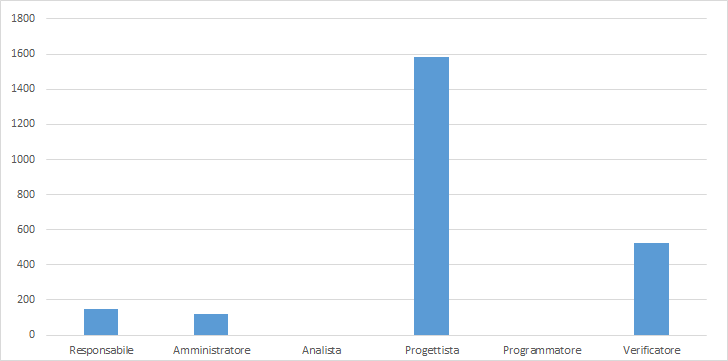
\includegraphics[scale=0.6]{img/8-3.png}
	\caption{Incidenza costi, Progettazione Architetturale Dettagliata}
\end{figure}

\newpage
\subsection{Codifica}
Il prospetto economico per quanto concerne la Codifica è il seguente:


\begin{table}[H]
	\begin{center}
		\begin{tabular}{|c|c|c|c|}
			\hline
			\textbf{Ruolo}	& \textbf{Numero di ore} & \textbf{Costo} & \textbf{Costo a preventivo}\\
			\hline
			\Res	&	6  &	180  &	180	\\
			\hline
			\Amm	&	3  &	60  &	60	\\
			\hline
			\Progr	&	143  &	2145  &	2145	\\
			\hline
			\Ver	&	61  &	915  &	915		\\
			\hline
			\textbf{Totale}  &	\textbf{213} &	\textbf{3300} &	\textbf{3300}	\\
			\hline
		\end{tabular}
	\end{center}
	\caption{Prospetto dei costi, Codifica }
\end{table}

\begin{figure}[H]
	\centering
	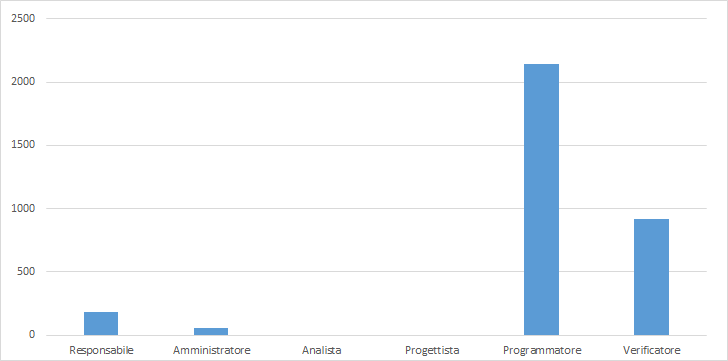
\includegraphics[scale=0.6]{img/8-4.png}
	\caption{Incidenza costi, Codifica}
\end{figure}

\newpage
\subsection{Verifica e Validazione}
Il prospetto economico per quanto concerne la fase di verifica e validazione è il seguente:


\begin{table}[H]
	\begin{center}
		\begin{tabular}{|c|c|c|c|}
			\hline
			\textbf{Ruolo}	& \textbf{Numero di ore} & \textbf{Costo} & \textbf{Costo a preventivo}\\
			\hline
			\Res	&	3  &	90  &	90	\\
			\hline
			\Amm	&	3  &	60  &	60	\\
			\hline
			\Prog	&	15  &	330  &	330	\\
			\hline
			\Ver	&	78  &	1170  &	1170	\\
			\hline
			\textbf{Totale}  &	\textbf{99}  &	\textbf{1680}  &	\textbf{1680}	\\
			\hline
		\end{tabular}
	\end{center}
	\caption{Prospetto dei costi, Verifica e Validazione}
\end{table}

\begin{figure}[H]
	\centering
	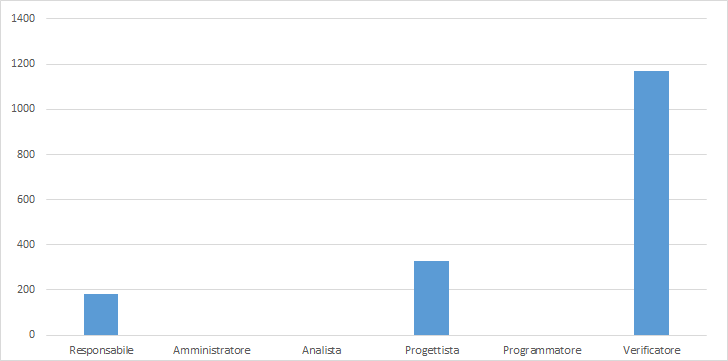
\includegraphics[scale=0.6]{img/8-5.png}
	\caption{Incidenza costi, Verifica}
\end{figure}

\newpage
\subsection{Consuntivo totale e considerazioni conclusive}

Di seguito, la tabella mostra totale delle ore rendicontate, con il costo parziale e complessivo, suddiviso per ruolo. 

\begin{table}[H]
	\begin{center}
		\begin{tabular}{|c|c|c|}
			\hline
			\textbf{Ruolo}	& \textbf{Ore rendicontabili} & \textbf{Costo} \\
			\hline
			\Res	&	19  &	570	\\
			\hline
			\Amm	&	17  &	340	\\
			\hline
			\Prog	&	225  &	4950	\\
			\hline
			\Progr	&	143  &	2145	\\
			\hline
			\Ver	&	226  &	3390	\\
			\hline
			\textbf{Totale}  & \textbf{630}  &	\textbf{11395}	\\
			\hline
		\end{tabular}
	\end{center}
	\caption{Prospetto dei costi complessivo}
\end{table}

\begin{figure}[H]
	\centering
	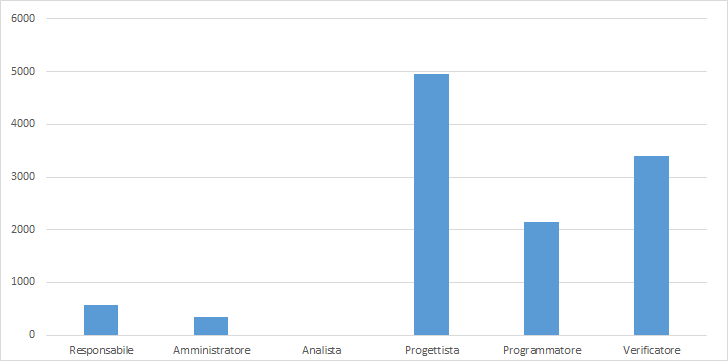
\includegraphics[scale=0.6]{img/8-6.png}
	\caption{Incidenza costi complessiva}
\end{figure}

Il costo complessivo preventivato per la realizzazione del progetto è, quindi, di \textbf{€ 11395}.